\section{Turing Machine}

While finite state automata and pushdown automata are all valid models of computation, they are too restricted as models of general purpose computers. Our goal is to have a model so that we can define computation as abstractly and general as possible.

How do we define algorithms rigorously? What does it mean for an algorithm to run in polynomial time. How do we argue that efficient algorithms do not exist.

Turing machine is a model of computation first proposed by Alan Turing in 1936. It is much more powerful than previous models that we have looked at. It is sufficiently general and can model what a human can do. A Turing machine can be think of a finite automata with unlimited and unrestricted memory.

In a Turing machine, we have an \textbf{one-way infinite tape} divided into ``cells'', each holding one symbol, including the blank symbol $\sqcup$. It also has a \textbf{read-write} head positioned in one square at a time that can move to the left or right. The control of the Turing is in of a fixed number of states. (The blank symbol $\sqcup$ is sometimes denoted by $\not b$ or $\square$ )

Initially, the input tape contains a finite number of symbols starting at the left-most cell with the remaining cells blank. The head starts at the left-most input symbol. Current state and symbol determine the next state, symbol written, and the movement of the head (either one square left or one square right).

\begin{figure}[htbp]
    \centering
    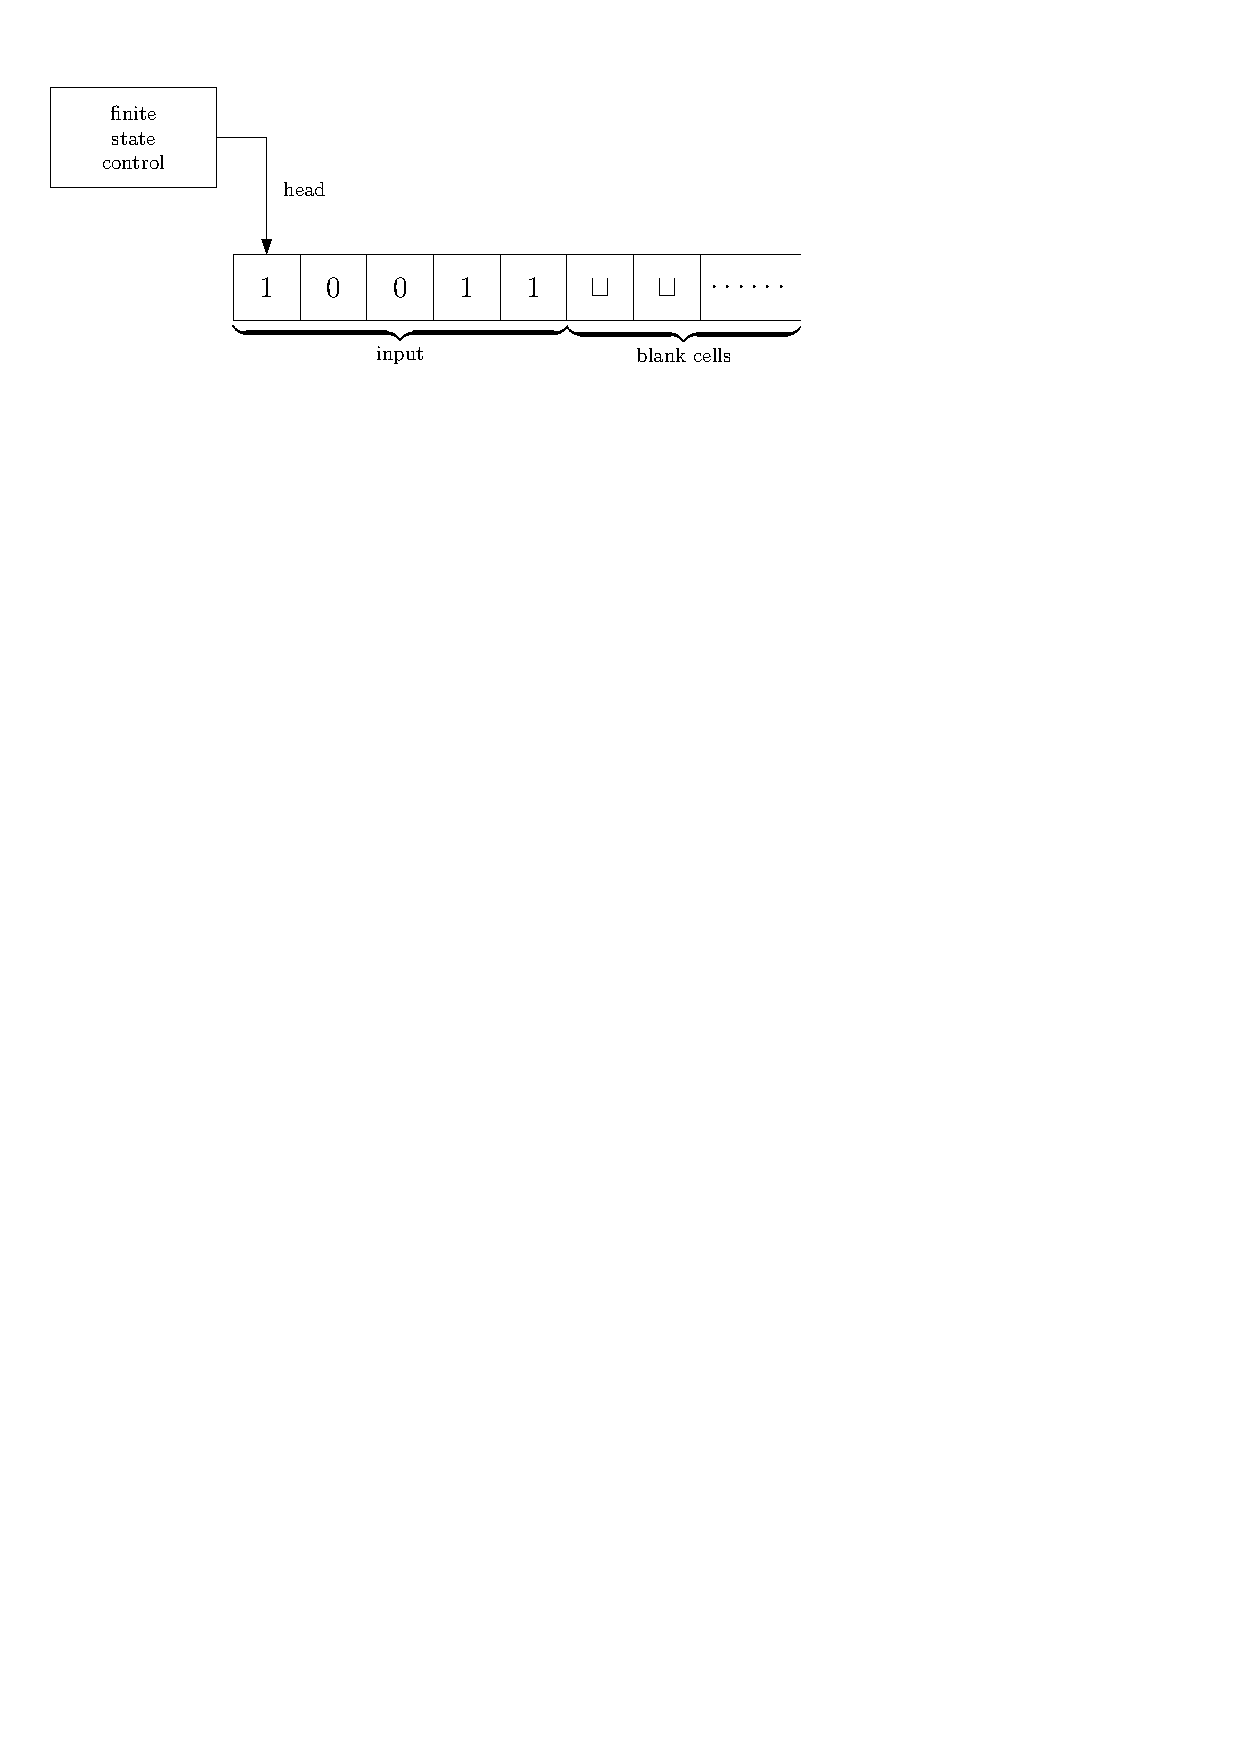
\includegraphics[width=0.7\linewidth]{tm.pdf}
    \caption{A Turing machine}
    \label{fig:tm}
\end{figure}

\begin{definition}[Turing Machine]
    A Turing machine is a 7-tuple $(Q,\Sigma,\Gamma,\delta,q_0,q_{accept},q_{reject})$ where $Q,\Sigma,\Gamma$ are all finite sets, and
    \begin{itemize}
        \item $Q$ is the set of states
        \item $\Sigma$ is the input alphabet not containing the blank symbol $\sqcup$
        \item $\Gamma$ is the tape alphabet, where $\sqcup \in \Gamma$ and $\Sigma \subset \Gamma$
        \item $\delta:\;(Q-\{q_{accept},q_{reject}\}) \times \Gamma \to Q \times \Gamma \times \{L,R\}$ is the transition function
        \item $q_0 \in Q$ is the start state
        \item $q_{accept} \in Q$ is the accept state
        \item $q_{reject} \in Q$ is the reject state, where $q_{accept} \neq q_{reject}$ 
    \end{itemize}
\end{definition}

$\delta(q,a) = (q',a',x)$ where $x \in \{L,R\}$ means if a machine is in state $q$ and head positioned on a square containing $a$, then the machine replaces $a$ with $a'$, moves to state $q$, and moves the head left ($L$) or right ($R$) depending on the direction given by $x$.

A Turing machine $M$ works as follows on input string $x \in \Sigma^*$.
\begin{enumerate}
    \item Initially $x = x_1x_2\ldots x_n \in \Sigma^*$ appears on leftmost $n$ squares of the input tape. Rest of the tape is blank;
    \item Head of $M$ starts on the leftmost square of tape;
    \item Initial state is $q_0$ 
    \item $M$ moves according to the transition function $\delta$
    \item Continue until $M$ reaches $q_{accept}$ or $q_{reject}$ and then $M$ halts. Otherwise, continue on forever.
\end{enumerate}

\begin{definition}[Language Recognized by Turing Machine]
    We say a Turing machine $M$ \textbf{accepts} a string $x \in \Sigma^*$ if $M$ upon reading the input $x$ eventually \textbf{halts} in state $q_{accept}$.

    Let $L(M) = \{x \in \Sigma^* \mid \text{$M$ accepts $x$} \}$. We say $L(M)$ is the \textbf{language recognized/accepted by} $M$. We say $x \not\in L(M)$ if $M$ upon reading $x$ either \textbf{halts} in $q_{reject}$ or \textbf{loops}.
\end{definition}

\begin{example}[Palindrome]
    $$\mathrm{Palindrome} = \{yy^R \mid y \in \{0,1\}^*\}$$
    At a high level, the \textbf{Turing machine} that decides this language scans back and forth, matching and erasing leftmost and rightmost symbols. Accept if the input is completely earased or reject if otherwise.
\end{example}

\section{Configuration of Turing Machine}

The \textbf{configuration} of a Turing machine describes the state, head position, and tape contents. It is denoted $x q y$ where $x,y \in \Gamma^*$ and $q \in  Q$. In this notation, the head position is implied to be the leftmost symbol of $y$.

Note that $xqy$ and $xqy \sqcup$ are equivalent configurations, but $xqy$ and $\sqcup xqy$ are not equivalent. Whether or not the first symbol is blank is important.

\begin{definition}
    Given two configurations $C_1$ and $C_2$, we say configuration $C_1$ \textbf{yields} $C_2$ if $C_2$ follows from $C_1$ by one step of $M$ (one application of $\delta$).
\end{definition}

\begin{example}
    Let $x,y \in \Gamma^*$ and $a,b \in \Gamma$. If $\delta(q,a) = (q',a',R)$, then $xqay$ yields $xa'q'y$. If $\delta(q,b) = (q',b',L)$, then $xaqby$ yields $xq'ab'y$. $qby$ yields $q'b'y$ because the tape head cannot move left anymore.
\end{example}

\begin{definition}[Computation]
    The \textbf{computation} of $M$ on input $x \in \Sigma^*$ is the sequence $C_0C_1C_2\ldots$ where $C_0 = q_0x$ and each configuration follows from the previous one. We say the computation is \textbf{halting} if it eventually reaches accept or reject state. Otherwise, we say the computation is \textbf{looping} (infinite).
\end{definition}

\section{Decidability and Recognizability}

\begin{definition}[Decider]
    A Turing machine $M$ is a decider if it halts on all inputs $x \in \Sigma^*$.
\end{definition}

\begin{definition}[Turing Decidable and Turing Recognizable]
    A language $A \in \Sigma^*$ is Turing decidable if and only if there is a \textbf{decider} $M$ such that $L(M)=A$.

    $A$ is semidecidable/Turing recognizable if and only if there is a Turing machine $M$ such that $L(M)=A$. In this case, $M$ may not halt if it does not accept $A$ (reject by looping).
\end{definition}

\section{Some Classes of Languages}

$\textsf{D} = \{ A \subseteq \Sigma^* \mid \text{$A$ is decidable}$

$\textsf{SD} = \{A \subseteq \Sigma^* \mid \text{$A$ is semidecidable}$

$\textsf{P} = \{A \subseteq \Sigma^* \mid \text{$A=L(M)$ for some $M$ that halts in polynomial time} \}$

Later, we will show that $\textsf{P} \subsetneq \textsf{D} \subsetneq \textsf{SD}$.

\section{Difference Between FSA and TM}

\begin{itemize}
    \item TM can read and write symbols. Infinite tape.
    \item Head can move left or right, unless the head is at left-most position.
    \item Special ``accept'' and ``reject'' states that stop computation immediately. The machine halts only when it reaches an accept or reject state. On the other hand, an FSA can only perform a finite amount of transitions before it halts.
\end{itemize}